
\renewcommand{\summarizedlecture}{8 }


%
%
%

\begin{frame}{Lecture \summarizedlecture revision (Conductors moving in a magnetic field)}

\begin{columns}
  \begin{column}{0.50\textwidth}
     We consider a conductor with length L moves with velocity $\vec{u}$ inside a
     homogenous magnetic field $\vec{B}$, as shown on the right.
  \end{column}
  \begin{column}{0.50\textwidth}
   \begin{center}
     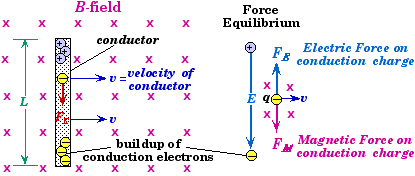
\includegraphics[width=0.90\textwidth]{./images/schematics/conductor_in_magnetic_field_induced_emf.png}\\
   \end{center}
  \end{column}
\end{columns}

\vspace{0.2cm}

Each electron in the conductor feels a magnetic force $\vec{F}_{M} = q \vec{u} \times \vec{B}$.\\
\vspace{0.1cm}
That magnetic force {\bf induces the build-up of charge}
which {\bf produces an electric field} $\vec{E}$:
Each electron feels an electric force $\vec{F}_{E} = q \vec{E}$.\\
\vspace{0.2cm}
The resulting {\bf electric force} $\vec{F}_{E}$ {\bf opposes the magnetic force} $\vec{F}_{M}$.\\

\vspace{0.2cm}

An electrical potential difference develops between the ends of the moving conductor,
which becomes a source of EMF:
\begin{equation*}
   \mathcal{E} = \int_{L} \vec{E} \cdot d\vec{\ell} = \int_{L} \Big( \vec{u} \times \vec{B} \Big) \cdot d\vec{\ell}
\end{equation*}

\end{frame}

%
%
%

\begin{frame}{Lecture \summarizedlecture revision  (Circuit moving in a magnetic field)}

A rectangular circuit moving through a region with magnetic field $\vec{B}$:
\begin{center}
  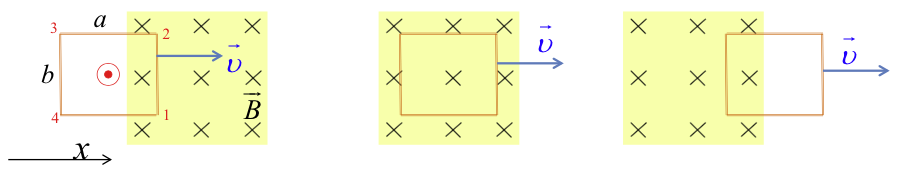
\includegraphics[width=0.88\textwidth]{./images/schematics/circuit_moving_through_magnetic_field_all_3.png}
\end{center}

\begin{columns}
  \begin{column}{0.55\textwidth}
  In summary:
  {\small
    \setlength{\extrarowheight}{10pt}
    \setlength{\arraycolsep}{5pt}
    \begin{table}[H]
        \begin{tabular}{|c||c|c|}
        \hline
               & $\displaystyle \oint_{L} \vec{E} \cdot d\vec{\ell}$ & $\displaystyle \frac{d\Phi_{M}}{dt}$\\
        \hline
          left   &  uBb &  -uBb \\
          centre & 0    &  0   \\
          right  &  -uBb & uBb \\
        \hline
        \end{tabular}
    \end{table}
  }
  \end{column}
  \begin{column}{0.45\textwidth}
     So, indeed, in all cases:
     \begin{equation*}
       \mathcal{E} = \oint_{L} \vec{E} \cdot d\vec{\ell} = - \frac{d\Phi_{M}}{dt}
     \end{equation*}
  \end{column}
\end{columns}

\end{frame}

%
%
%

\begin{frame}{Lecture \summarizedlecture revision (Faraday's observations)}

In 1831 Michael Faraday reported on a series of experiments.\\
\vspace{0.2cm}

A current flows in a wire loop when:
\vspace{0.1cm}
\begin{enumerate}[(a)]
{\small
  \item the loop is pulled through a magnetic field,
  \item the loop is at rest but the magnet moves in the opposite direction, and
  \item both the loop and the magnet are at rest but the strength of the magnetic field is varied
}
\end{enumerate}

\begin{center}
  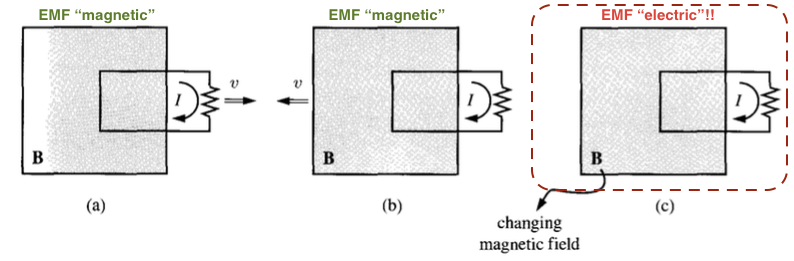
\includegraphics[width=0.80\textwidth]{./images/schematics/faraday_law_schematic_with_notes.png}
\end{center}
This led Faraday to realize that:
\begin{center}
{\bf A time-varying magnetic field induces an electic field}
\end{center}

\end{frame}

%
%
%

\begin{frame}{Lecture \summarizedlecture revision (Faraday's law / Lenz's law)}

In all cases the {\bf motional EMF} is directly related
to the {\bf change of the magnetic flux $\Phi_{M}$ though the circuit}:\\

\vspace{0.1cm}

\begin{columns} [T]
  \begin{column}{0.25\textwidth}
    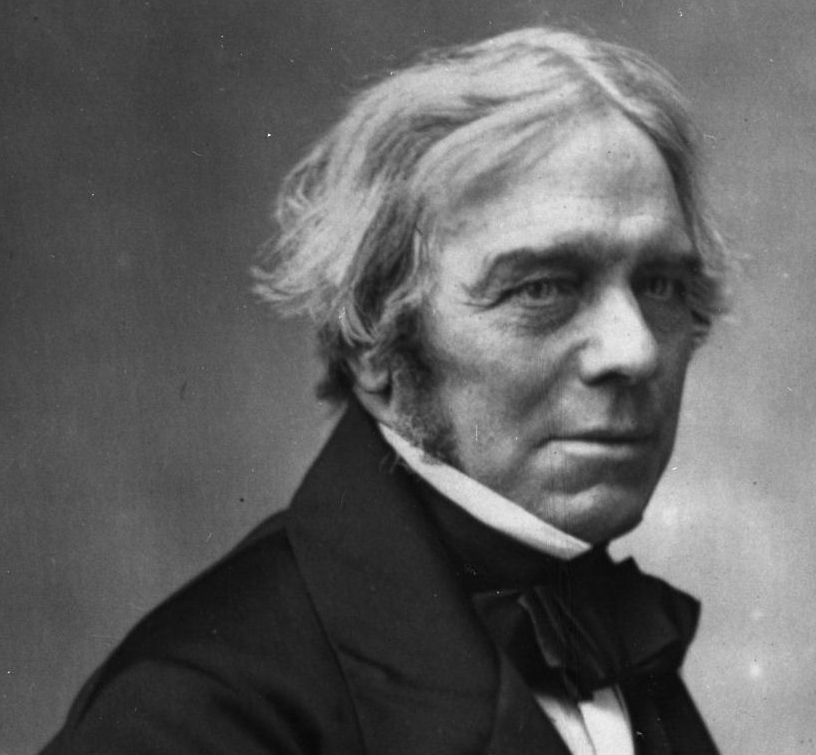
\includegraphics[width=0.98\textwidth]{./images/people/faraday.png}\\
    {\tiny Michael Faraday (1791 - 1867).}
  \end{column}
  \begin{column}{0.75\textwidth}
   \begin{center}
    \begin{equation*}
      \mathcal{E} = \oint_{L} \vec{E} \cdot d\vec{\ell} = - \frac{d\Phi_{M}}{dt}
    \end{equation*}
    \vspace{0.2cm}
    This is the so-called {\bf Faraday's law}.
   \end{center}
  \end{column}
\end{columns}

\vspace{0.1cm}

\begin{columns}
  \begin{column}{0.75\textwidth}
  {\scriptsize
    Lenz' law (1845): The EMF induced by a changing flux has a polarity
    such that the current flowing gives rise to a flux which opposes the change of flux.\\
    \vspace{0.1cm}
    The minus sign is a consequence of the {\bf conservation of energy} and
    of {\bf Newton's 3rd law} of motion: Induction is a an ``inertial reaction''.
    The system develops a current which tries to maintain the flux constant.\\
  }
  \end{column}
  \begin{column}{0.25\textwidth}
    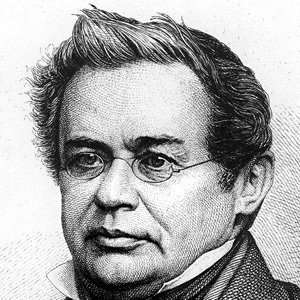
\includegraphics[width=0.83\textwidth]{./images/people/lenz.jpg}\\
    {\tiny Heinrich Lenz (1804 - 1865).}
  \end{column}
\end{columns}

\end{frame}

%
%
%

\begin{frame}{Lecture \summarizedlecture revision (Maxwell correction in Ampere's law)}

We also studied a case where Ampere's law led to paradoxical results.\\

\vspace{0.2cm}

We also saw that Ampere's law (as we knew it) was inconsistent with
the continuity equation (which expresses the local conservation of charge).\\

\vspace{0.2cm}

The problem of course was that we took a law from magnetostatics and
applied it in a different context (electrodynamics) where it is no longer valid.

\vspace{0.2cm}

Maxwell realised that all it takes to fix Ampere's law is to do the following substitution:
\begin{equation*}
  \vec{j} \rightarrow
  \vec{j} + \epsilon_0 \frac{\partial \vec{E}}{\partial t}
\end{equation*}

The term $\displaystyle \epsilon_0 \frac{\partial \vec{E}}{\partial t}$
is called {\bf displacement current}.

\end{frame}

%
%
%

\begin{frame}{Lecture \summarizedlecture revision (Maxwell's eqs for the dynamic case)}

Compared with what we had seen in the study of electrostatics and magnetostatics,
the study of time-dependent fields (electrodynamics) brought the following complication:\\

\vspace{0.1cm}

\begin{itemize}
   \item {\bf Electric fields are produced} not only by electric charges,
             but also {\bf by changing magnetic fields!}
     \begin{equation*}
        \vec{\nabla} \times \vec{E} = {\color{red} - \frac{\partial \vec{B}}{\partial t}}
     \end{equation*}

   \item {\bf Magnetic fields are produced} not only by electric currents,
             but also {\bf by changing electric fields!}
     \begin{equation*}
         \vec{\nabla} \times \vec{B} = \mu_{0} \Big( \vec{j} + {\color{red} \epsilon_0 \frac{\partial \vec{E}}{\partial t} } \Big)
     \end{equation*}
\end{itemize}

{\small
The full list of Maxwell equations for the static and dynamic cases in vacuum is shown on the next slide.
Notice that all 4 equations are coupled in the dynamic case.\\
}

\end{frame}

%
%
%

\begin{frame}{Lecture \summarizedlecture revision (Maxwell's eqs. for the dynamic case)}

{\small

\begin{center}
{
  \begin{table}[H]
    \begin{tabular}{|l|c|c|}
      \hline
        \multicolumn{3}{|l|} {
          {\color{magenta}
           {\bf Static case (in vacuum)}
          }
        }\\
      \hline
      {\bf Gauss's law} &
        $\displaystyle \oint \vec{E} d\vec{S} = \frac{1}{\epsilon_0} \int \rho d\tau$ &
        $\displaystyle \vec{\nabla} \cdot \vec{E} = \frac{\rho}{\epsilon_0}$ \\

      {\bf Circuital law} &
        $\displaystyle \oint \vec{E} d\vec{\ell} = 0$ &
        $\displaystyle \vec{\nabla} \times \vec{E} = 0$ \\

      no magn. monopoles' &
        $\displaystyle  \oint \vec{B} d\vec{S} = 0$ &
        $\displaystyle  \vec{\nabla} \cdot \vec{B} = 0$ \\

      {\bf Ampere's law} &
        $\displaystyle \oint \vec{B} d\vec{\ell} = \mu_{0} \int \vec{j} d\vec{S}$ &
        $\displaystyle \vec{\nabla} \times \vec{B} = \mu_{0} \vec{j}$ \\
      \hline
    \end{tabular}
  \end{table}
}
\end{center}


\begin{center}
{
  \begin{table}[H]
    \begin{tabular}{|l|c|c|}
      \hline
        \multicolumn{3}{|l|} {
          {\color{magenta}
           {\bf Generalization of above for the dynamic case (in vacuum)}
          }
        }\\
      \hline
      {\bf Gauss's law} &
        $\displaystyle \oint \vec{E} d\vec{S} = \frac{1}{\epsilon_0} \int \rho d\tau$ &
        $\displaystyle \vec{\nabla} \cdot \vec{E} = \frac{\rho}{\epsilon_0}$ \\

      {\bf Circuital law} &
        $\displaystyle \oint \vec{E} d\vec{\ell} =  -\frac{\partial}{\partial t} \int \vec{B} d\vec{S}$ &
        $\displaystyle \vec{\nabla} \times \vec{E} = -  \frac{\partial \vec{B}}{\partial t}$ \\

      no magn. monopoles &
        $\displaystyle  \oint \vec{B} d\vec{S} = 0$ &
        $\displaystyle  \vec{\nabla} \cdot \vec{B} = 0$ \\

      {\bf Ampere's law} &
        $\displaystyle \oint \vec{B} d\vec{\ell} = \mu_{0} \int \Big( \vec{j} + \epsilon_0 \frac{\partial \vec{E}}{\partial t}\Big) d\vec{S}$ &
        $\displaystyle \vec{\nabla} \times \vec{B} = \mu_{0} \Big( \vec{j} + \epsilon_0 \frac{\partial \vec{E}}{\partial t}\Big)$ \\
      \hline
    \end{tabular}
  \end{table}
}
\end{center}

}
\end{frame}



%
%
%

\begin{frame}{Lecture \summarizedlecture - \lecturesummarytitle}

Compared with what we had seen in the study of electrostatics and magnetostatics,
the study of time-dependent fields (electrodynamics) brought the following complication:\\

\vspace{0.1cm}

\begin{itemize}
   \item {\bf Electric fields are produced} not only by electric charges,
             but also {\bf by changing magnetic fields!}
     \begin{equation*}
        \vec{\nabla} \times \vec{E} = {\color{red} - \frac{\partial \vec{B}}{\partial t}}
     \end{equation*}

   \item {\bf Magnetic fields are produced} not only by electric currents,
             but also {\bf by changing electric fields!}
     \begin{equation*}
         \vec{\nabla} \times \vec{B} = \mu_{0} \Big( \vec{j} + {\color{red} \epsilon_0 \frac{\partial \vec{E}}{\partial t} } \Big)
     \end{equation*}
\end{itemize}

{\small
The full list of Maxwell equations for the static and dynamic cases in vacuum is shown on the next slide.
Notice that whereas the 2 equations involving $\vec{E}$ and the 2 equations involving $\vec{B}$ were decoupled in the static case,
all 4 equations are coupled in the dynamic case.\\
}

\end{frame}


%
%
%

\begin{frame}{Maxwell's equations for the static and dynamic cases}

{\small

\begin{center}
{
  \begin{table}[H]
    \begin{tabular}{|l|c|c|}
      \hline
        \multicolumn{3}{|l|} {
          {\color{magenta}
           {\bf Static case (in vacuum)}
          }
        }\\
      \hline
      {\bf Gauss's law} &
        $\displaystyle \oint \vec{E} d\vec{S} = \frac{1}{\epsilon_0} \int \rho d\tau$ &
        $\displaystyle \vec{\nabla} \cdot \vec{E} = \frac{\rho}{\epsilon_0}$ \\

      {\bf Circuital law} &
        $\displaystyle \oint \vec{E} d\vec{\ell} = 0$ &
        $\displaystyle \vec{\nabla} \times \vec{E} = 0$ \\

      no magn. monopoles' &
        $\displaystyle  \oint \vec{B} d\vec{S} = 0$ &
        $\displaystyle  \vec{\nabla} \cdot \vec{B} = 0$ \\

      {\bf Ampere's law} &
        $\displaystyle \oint \vec{B} d\vec{\ell} = \mu_{0} \int \vec{j} d\vec{S}$ &
        $\displaystyle \vec{\nabla} \times \vec{B} = \mu_{0} \vec{j}$ \\
      \hline
    \end{tabular}
  \end{table}
}
\end{center}


\begin{center}
{
  \begin{table}[H]
    \begin{tabular}{|l|c|c|}
      \hline
        \multicolumn{3}{|l|} {
          {\color{magenta}
           {\bf Generalization of above for the dynamic case (in vacuum)}
          }
        }\\
      \hline
      {\bf Gauss's law} &
        $\displaystyle \oint \vec{E} d\vec{S} = \frac{1}{\epsilon_0} \int \rho d\tau$ &
        $\displaystyle \vec{\nabla} \cdot \vec{E} = \frac{\rho}{\epsilon_0}$ \\

      {\bf Circuital law} &
        $\displaystyle \oint \vec{E} d\vec{\ell} =  -\frac{\partial}{\partial t} \int \vec{B} d\vec{S}$ &
        $\displaystyle \vec{\nabla} \times \vec{E} = -  \frac{\partial \vec{B}}{\partial t}$ \\

      no magn. monopoles &
        $\displaystyle  \oint \vec{B} d\vec{S} = 0$ &
        $\displaystyle  \vec{\nabla} \cdot \vec{B} = 0$ \\

      {\bf Ampere's law} &
        $\displaystyle \oint \vec{B} d\vec{\ell} = \mu_{0} \int \Big( \vec{j} + \epsilon_0 \frac{\partial \vec{E}}{\partial t}\Big) d\vec{S}$ &
        $\displaystyle \vec{\nabla} \times \vec{B} = \mu_{0} \Big( \vec{j} + \epsilon_0 \frac{\partial \vec{E}}{\partial t}\Big)$ \\
      \hline
    \end{tabular}
  \end{table}
}
\end{center}

}
\end{frame}
